\subsection{Differenziabilità}

\subsubsection{Differenza tra derivabilità e differenziabilità}

Il fatto che la funzione a \textbf{una variabile} sia derivabile in un punto mi dice che esiste la retta tangente in quel punto.

Per le funzioni a due variabili questo non è vero, infatti, per le funzioni a più di una variabile:
\[\text{derivabilità} \ne \text{differenziabilita}\]

Questo è dato dal fatto che per le funzioni in due variabili la derivabilità non implica la continuità:

\[
    derivabile \centernot\implies continua
\]

\textbf{Controesempio}

Calcolare, se esistono, le derivate parziali in \((0,0)\):

\[
    f(x,y)=
    \begin{cases}
        \frac{xy^{2}}{x^{2}+y^{4}} & \text{se}\ (x,y)\neq (0,0) \\
        0                          & \text{se}\ (x,y)=(0,0)
    \end{cases}
\]

Consideriamo le tracce:

\[
    f(x,0) = 0 \quad;\quad f(0,y) =0
\]

Dunque ottengo due funzioni identicamente nulle che sono derivabili con derivata nulla:

\[
    f_x(0,0) = f_y(0,0) = 0
\]

Osserviamo però che in \((0,0)\) la funzione non è continua perché:

\[
    \lim_{ (x,y) \to (0,0) } \frac{xy^{2}}{x^{2}+y^{4}} \text{ non esiste}
\]

Per risolvere questo problema, quello che ci servirà sarà il concetto di \textbf{differenziabilità}.

\filbreak{}
\subsubsection{Definizione di differenziabilità}

Avendo una funzione \(f:A\subseteq \Rn  \rightarrow \R \) con \(A\) aperto

f è derivabile in \(\ux =(x_1, \ldots ,x_n) \in A\) equivale a dire che esiste il vettore gradiente:

\[
    \nabla f(\ux ) = \left( \frac{\partial f}{\partial x_1}(\ux ), \ldots , \frac{\partial f}{\partial x_n}(\ux ) \right)
\]

\defn{Differenziabilità}{
Il concetto di differenziabilità è più forte rispetto al concetto di derivabilità.

Infatti, si dice che \(f\) è differenziabile in \(\ux \in A \) se \(f\) è derivabile in \(\ux \) e inoltre vale la seguente relazione:

\[
    \lim_{ \uh \to 0 } \frac{f( \ux + \uh ) - f( \ux ) - \langle  \nabla f(\ux ), \uh \rangle}{\norm{\uh}} =0
\]

dove \(\uh \in \Rn \); e inoltre ricordo che:

\[
    \norm{\uh} = \sqrt{\sum^{n}_{i=1} h_i^{2}}
\]

\[
    \langle  \nabla f(\ux ), \uh \rangle = \frac{\partial f}{\partial x_1}(\ux )\cdot h_1+ \frac{\partial f}{\partial x_2}(\ux ) \cdot h_2+ \cdots  + \frac{\partial f}{\partial x_n}(\ux ) \cdot h_n
\]

Se \(f\) è differenziabile in ogni punto di \(A\) si dice che \(f\) è differenziabile in \(A\)
}

Da notare che il prodotto scalare \(\langle \nabla f(\ux ), \uh  \rangle \) rappresenta l'incremento che io faccio verso ogni direzione per poter ``vedere'' che cosa succede quando mi sposto un ``pochino'' in ogni direzione.

\defn{Differenziale}{
    Definisco come \(L : \Rn  \rightarrow \R \) l'applicazione che ad \(\uh \) associa il prodotto scalare:

    \[
        \uh \mapsto \langle  \nabla f(\ux ) , \uh \rangle
    \]

    Questa applicazione si chiama \textbf{differenziale} di \(f\) in \(\ux \) e si indica con \(\diff f(\ux)\)

    Questa è un'\textbf{applicazione lineare} da \(\Rn \) in \(\R \) della variabile \(\uh \)

    \[
        \diff f(\ux ) (\uh ) = \langle \nabla f(\ux ) , \uh  \rangle
    \]
}

\filbreak{}
Usando questa nomenclatura, possiamo dunque dire che \(f\) è differenziabile in \(\ux \in A\) se esiste un \textbf{funzionale lineare} \(L: \Rn \rightarrow \R \) tale che:

\[
    \lim_{ \uh \to 0 } \frac{f(\ux+\uh) -f(\ux) - L(\uh)}{\norm{\uh}} = 0
\]

In \(\Rn \) ogni funzionale lineare si rappresenta come un opportuno prodotto scalare.


Se \(L: \Rn \rightarrow \R \) è lineare allora esiste \(\underline{l} \in \Rn \) tale che:

\[
    L(\uh ) = \langle \uh , \underline{l} \rangle \quad \forall \uh \in \Rn
\]

Dunque, \(f: A \subseteq \Rn \rightarrow \R \) è differenziabile in \(\ux \in A\) se è derivabile in \(\ux \) e se:

\[
    f(\ux + \uh ) \xrightarrow[\uh \to 0]{} f(\ux ) + \langle \nabla f(\ux ), \uh  \rangle + o(\norm{\uh})
\]

\subsubsection{Significato geometrico del differenziale}

La differenziabilità è legata all'esistenza del piano tangente al grafico della \(f: A \subseteq \Rn \to \R \) in un punto \(\ux_0\).

Supponiamo che \(f\) sia differenziabile in \(\ux_0 \in A \), allora, tornando alla relazione definita dalla differenziabilità, per \(\uh \to 0\):

\[
    f(\ux_0+\uh) = f(\ux_0) +\langle \nabla f(\ux_0) , \uh \rangle  + o(\norm{\uh} )
\]

riscrivendolo per \(\uh = \ux - \ux_0\):

\[
    f(\ux) = \underbrace{f(\ux_0)}_{\begin{smallmatrix}\text{punto di} \\ \text{partenza}\end{smallmatrix}} + \underbrace{\langle \nabla f(\ux_0), \ux-\ux_0 \rangle}_\text{il mio spostamento} + \underbrace{o(\norm{\ux-\ux_0})}_{\begin{smallmatrix}\text{l'errore commesso} \\ \text{spostandosi}\end{smallmatrix}}
\]

e dunque la funzione lineare che associa:
\[\ux \mapsto  f(\ux_0 ) + \langle \nabla f(\ux_0 ), \ux-\ux_0 \rangle \]
ci fornisce un'\textbf{approssimazione di tipo lineare} della \(f(\ux)\) nel punto \(\ux_0\) a meno di infinitesimi di ordine superiore alla distanza euclidea tra \(\ux \) e \(\ux_0\):

\[
    d(\ux,\ux_0) = \norm{\ux-\ux_0}
\]

\textbf{Importante}:

Il grafico di questa funzione lineare rappresenta il piano tangente al grafico di \(f\) nel punto \(\ux_0\) in cui la \(f\) è differenziabile.

Per \(n=2\) ritroviamo infatti l'equazione vista in precedenza del piano tangente al punto \(\ux_0\).

Questo è chiaro in due variabili perché ci spostiamo sia lungo le \(x\) che le \(y\) e quindi disegniamo un piano.

\pagebreak
\subsubsection{Differenziale come approssimazione lineare (per n=2)}

Consideriamo:

\[
    \underline{P_0} = (x_0,y_0)
\]

con \(f\) differenziabile in \(\underline{P_0}\).

L'equazione del piano tangente al grafico di \(f\) nel punto \(\underline{P_0}\) è:

\[
    z= f(\underline{P_0}) + \langle \nabla f(\underline{P_0}), \underline{P}-\underline{P_0} \rangle
\]

ovvero, sapendo che:

\[
    \nabla f(\underline{P_0}) = \left( \frac{\partial f}{\partial x}(x_0,y_0), \frac{\partial f}{\partial y}(x_0,y_0) \right)
\]

allora l'equazione del piano tangente nel punto (\(x_0,y_0,f(x_0,y_0)\)) diventa:

\[
    z = f(x_0,y_0) + \frac{\partial f}{\partial x}(x_0,y_0) (x-x_0) + \frac{\partial f}{\partial y}(x_0,y_0) (y-y_0)
\]

Scriviamo la definizione di differenziale in \(\uh=(h_x,h_y)\) per \((h_x,h_y) \rightarrow (0,0)\):

\[
    f(x_0+h_x,y_0+h_y) = f(x_0,y_0) + \frac{\partial f}{\partial x}(x_0,y_0) \cdot h_x + \frac{\partial f}{\partial y}(x_0,y_0) \cdot h_y + \underbrace{ o\left( \sqrt{h_x^{2}+h_y^{2}} \right)}_{o(\norm{\uh})}
\]
\begin{equation*}
    \text{e se pongo }
    \begin{cases}
        x_0 + h_x = x \\
        y_0 + h_y = y
    \end{cases}
    \implies \text{allora:}
\end{equation*}

\[
    f(x,y) = f(x_0,y_0) + \frac{\partial f}{\partial x}(x_0,y_0) (x-x_0) + \frac{\partial f}{\partial y}(x_0,y_0) (y-y_0) + \underbrace{o\left( \sqrt{{(x-x_0)}^{2}+{(y-y_0)}^{2}} \right)}_\text{\(d(\underline{P},\underline{P}_0)\)}
\]

E dunque, per le funzioni differenziabili si ha che il piano di equazione:

\[
    z= f(x_0,y_0) + \frac{\partial f}{\partial x}(x_0,y_0)(x-x_0) + \frac{\partial f}{\partial y}(x_0,y_0) (y-y_0)
\]

dista dal grafico di \(f\) per una quantità che va a zero più rapidamente di quanto \(\underline{P}\) si avvicini a \(\underline{P}_0\).

\[
    f(x,y) - \left[ f(x_0,y_0) + \frac{\partial f}{\partial x}(x_0,y_0) (x-x_0) + \frac{\partial f}{\partial y}(x_0,y_0) (y-y_0) \right] = \underbrace{o\left( \sqrt{{(x-x_0)}^{2}+{(y-y_0)}^{2}} \right)}_\text{\(d(\underline{P},\underline{P}_0)\)}
\]

\filbreak{}
quindi:

\[
    \lim_{ (x,y) \to (x_0,y_0) } \frac{f(x,y) - \left[ f(x_0,y_0) + \frac{\partial f}{\partial x}(x_0,y_0) (x-x_0) + \frac{\partial f}{\partial y}(x_0,y_0) (y-y_0) \right] }{\sqrt{{(x-x_0)}^{2}+{(y-y_0)}^{2}}}= 0
\]

La funzione \(L: \R^{2} \rightarrow \R \):

\[
    L(x,y) = f(x_0,y_0) + \frac{\partial f}{\partial x}(x_0,y_0) (x-x_0) + \frac{\partial f}{\partial y}(x_0,y_0) (y-y_0)
\]

il cui grafico è il piano tangente al grafico di \(f\) in \((x_0,y_0)\), si chiama anche \textbf{linearizzazione} di \(f(x,y)\) in \((x_0,y_0)\).

L'applicazione delle \(f\) mediante tale piano viene detta \textbf{approssimazione lineare} della \(f\) in \((x_0,y_0)\)

\pagebreak
\subsubsection{Esempio di esercizio sulla differenziabilità}

Data la funzione:

\[
    f(x,y) = \begin{cases}
        \displaystyle \frac{x^{3}+2y^{4}}{x^{2}+y^{2}} & \text{se \((x,y) \neq (0,0)\)} \\
        0                                              & \text{se \((x,y) = (0,0)\)}
    \end{cases}
\]

\begin{enumerate}
    \item Stabilire in quali punti del piano è derivabile, calcolandone le derivate in tale caso
    \item Stabilire in quali punti del piano è differenziabile
    \item Stabilire il più grande aperto \(A \subseteq \R^{2}\) su cui \(f\) è \(C^{1}\)
\end{enumerate}

\textbf{Soluzione}

\begin{enumerate}
    \item Osserviamo che se \((x,y) \neq (0,0)\) non presenta problemi ed è sempre derivabile in quanto composizione di funzioni sempre derivabili (polinomi). Le sue derivate parziali sono:

          \begin{align*}
               & \frac{\partial f}{\partial x}(x,y) = \frac{3x^{2}(x^{2}+y^{2})-2x(x^{3}+2y^{4})}{{(x^{2}+y^{2})}^{2}}= \frac{x^{4}+3x^{2}y^{2}-4xy^{4}}{{(x^{2}+y^{2})}^{2}}     \\[3mm]
               & \frac{\partial f}{\partial y}(x,y) = \frac{8y^{3}(x^{2}+y^{2}) - 2y(x^{3}+2y^{4})}{{(x^{2}+y^{2})}^{2}} = \frac{4y^{5}+8x^{2}y^{3}-2x^{3}y}{{(x^{2}+y^{2})}^{2}}
          \end{align*}

          Controlliamo ora la derivabilità in \((0,0)\):

          \[
              f(0,y) = 2y^{2} \implies f_y(0,y) = 4y \implies f_y(0,0) = 0
          \]
          \[
              f(x,0) = x \implies f_x(x,0) = 1 \implies f_x(0,0) = 1
          \]

          Dunque è derivabile anche in \((0,0)\) e di conseguenza in tutto \(\R^2\).

    \item Bisogna vedere che cosa succede in \((0,0)\) che è l'unico punto problematico per la continuità di \(f(x,y)\).

          Per essere differenziabile in \((0,0)\) deve essere:

          \[
              f(x,y) - f(0,0) - \frac{\partial f}{\partial x}(0,0) (x-0) - \frac{\partial f}{\partial y}(0,0) (y-0) = o\left( \sqrt{x^{2}+y^{2}} \right)
          \]

          e quindi deve valere il seguente limite:

          \begin{align*}
              \lim_{ (x,y) \to (0,0) } \frac{ \frac{x^{3}+2y^{4}}{x^{2}+y^{2}}-0 -1(x-0) -0(y-0)}{\sqrt{x^{2}+y^{2}}}
               & = \lim_{ (x,y) \to (0,0) } \frac{x^3+2y^{4}-x(x^2+y^2)}{(x^{2}+y^{2}) {(x^{2}+y^{2})}^{ \frac{1}{2}}} \\
               & = \lim_{ (x,y) \to (0,0) } \frac{2y^{4}-xy^{2}}{{(x^{2}+y^{2})}^{ \frac{3}{2}}}
              = 0
          \end{align*}

          Noto che:

          \[
              \left|\frac{2y^{4}-xy^{2}}{{(x^{2}+y^{2})}^{ \frac{3}{2}}}\right| \le \left|\frac{2y^{4}}{{(x^{2}+y^{2})}^{ \frac{3}{2}}}\right| \le \left|2y^{4}\right| = 2y^4 \xrightarrow[(x,y) \to (0,0)]{} 0
          \]

          Quindi per il teorema del confronto abbiamo verificato che vale il limite, e che quindi la funzione è differenziabile anche in \((0,0)\).
    \item Tutto \(\R^2\)
\end{enumerate}

\pagebreak
\subsubsection{Definizione formale di differenziabilità}

\defn{Differenziabilità}{
    Sia \(f:A \subseteq \Rn \rightarrow \R \) una funzione, con \(A\) aperto, e sia \(\ux_0 \in A\).

    Si dice che \(f\) è differenziabile in \(\ux_0\) se \(\exists L:\Rn \rightarrow \R \) funzione lineare tangente a \(f\)  in \(\ux_0\) tale che:

    \[
        \lim_{ \uh \to 0 } \frac{f(\ux_0+\uh) - f(\ux_0) -L(\uh)}{\norm{\uh}} = 0
    \]

    dove \(L(\uh) = \langle \nabla f(\ux_0), \uh \rangle \)
}

\subsubsection{Teoremi sulla differenziabilità e continuità}

\teorema{}{
    Sia \(f: A \subset \Rn \to \R \); Sia inoltre \(\ux_0 \in A\);

    \(f\) è differenziabile in \(\ux_0 \implies f\) è continua in \(\ux_0 \)
}


\begin{proof}
    Per dimostrare che \(f\) è continua in \(\ux_0 \) devo far vedere che:

    \[
        \lim_{ \uh \to 0 } f(\ux_0 + \uh) = f( \ux_0 )
    \]

    \[
        \lim_{ \uh \to 0 } f(\ux_0 + \uh ) \overset{\text{differenziabile}}{=}
        \lim_{ \uh \to 0 } \left[ f(\ux_0) + \langle \nabla f(\ux_0), \uh \rangle + o(\norm{\uh}) \right]
    \]

    applichiamo la disuguaglianza di Cauchy-Schwarz:

    \[
        \langle \nabla f(\ux_0), \uh \rangle \le
        \Big|\langle \nabla f(\ux_0), \uh \rangle\Big| \le
        \norm{\nabla f(\ux_0)} \cdot \norm{\uh}
        \xrightarrow[\uh \to 0]{} 0
    \]

    quindi abbiamo che:

    \[
        \lim_{ \uh \to 0 } \left[ f(\ux_0) + \underbrace{\langle \nabla f(\ux_0),\uh \rangle}_\text{\(\rightarrow 0\)} + \underbrace{o(\norm{\uh})}_\text{\(\rightarrow 0\)} \right] = f(\ux_0)
    \]
\end{proof}

\pagebreak
\teorema{Teorema del differenziale totale}{
    Sia la funzione \(f: A \subseteq \Rn  \rightarrow \R \) derivabile in \(A\) con \(A\) aperto.

    Se le derivate parziali \(f_{x_1}, \ldots, f_{x_n}\) sono continue in \(\ux_0 \in A\) allora \(f\) è differenziabile in \(\ux_0 \)
}

\begin{proof}
    Per \(n=2\)

    Sia \(f = f(x,y)\) con \((x,y) \in A \subseteq \R^{2}\), e sia \(\uh = (h,k)\):
    \begin{align*}
        f(x+h,y+k) - f(x,y) & = f(x+h,y+k) + f(x,y+k) - f(x,y+k) - f(x,y)                                                                        \\
                            & = \underbrace{[f(x+h,y+k) - f(x,y+k) ]}_{f(b,y+k) - f(a,y+k)} + \underbrace{[f(x,y+k) - f(x,y)]}_{f(x,b) - f(x,a)}
    \end{align*}

    Applico il teorema di Lagrange sulle due quadre, per cui:
    \[
        \exists x_0 \in (x,x+h) \giventhat f(x+h,y)-f(x,y) = f'(x_0) \cdot [(x+h)-(x)]
    \]
    \[
        \exists y_0 \in (y,y+k) \giventhat f(x,y+k)-f(x,y) = f'(y_0) \cdot [(y+k)-(y)]
    \]
    Dunque:
    \begin{align*}
        f(x+h,y+k) - f(x,y) & = \frac{\partial f}{\partial x}(x_0,y+k) (x +h -x) + \frac{\partial f}{\partial y}(x,y_0) ( y + k -y) \\
                            & = \frac{\partial f}{\partial x}(x_0,y+k) h + \frac{\partial f}{\partial y}(x,y_0)k
    \end{align*}
    Ora, parto dalla definizione di differenziabilità per \(f\) in \((x+h,y+k)\) e sostituisco quanto ottenuto sopra:

    \[
        \frac{f(x+h,y+k) - f(x,y) - f_x(x,y)h - f_y(x,y) k}{\sqrt{h^{2}+k^{2}}} =
    \]

    \[
        = \frac{\left[ f_x(x_0,y+k) h + f_y(x,y_0) k \right] -f_x(x,y)h -f_y(x,y)k}{\sqrt{h^{2}+k^{2}}} =
    \]

    \[
        = \frac{[f_x(x_0,y+k) - f_x(x,y)] h + [f_y(x,y_0) - f_y(x,y)] k}{\sqrt{h^{2}+k^{2}}}
    \]

    metto tutto in valore assoluto e maggioro:
    \begin{align*}
        [\ldots] & \le \left|\frac{[f_x(x_0,y+k) - f_x(x,y)] h + [f_y(x,y_0) - f_y(x,y)] k}{\sqrt{h^{2}+k^{2}}}\right|                      \\
                 & \le |f_x(x_0,y+k) - f_x(x,y_0)| \frac{|h|}{\sqrt{h^{2}+k^{2}}} + | f_y(x,y_0) - f_y(x,y)| \frac{|k|}{\sqrt{h^{2}+k^{2}}} \\
                 & \le  |f_x(x_0,y+k) - f_x(x,y_0) | + |f_y(x,y_0) - f_y(x,y) |
    \end{align*}

    \filbreak{}
    Quando \((h,k) \rightarrow (0,0)\) succede che \((x_0,y_0) \rightarrow (x,y)\). Inoltre, essendo \(f_x\) e \(f_y\) continue in \((x,y)\):

    \[
        |\underbrace{f_x(x,y+k) - f_x(x,y)}_\text{\(\rightarrow 0\)} | + |\underbrace{f_y(x,y) - f_y(x,y)}_\text{\(\rightarrow 0\)} | \xrightarrow[\uh \to 0]{} 0
    \]

    Quindi \(f(\ux,\uy)\) è differenziabile in \(\ux_0\).

\end{proof}

\defn{Continuità di funzioni in più variabili}{
    Quindi una funzione \(g: A \subset \Rn  \rightarrow \R \) continua in \(A\), si dice di classe \(C^{0}\) e si scrive \(f \in C^{0}(A)\)

    Se la funzione è derivabile in \(A\) e se le derivate parziali sono continue in \(A\) si dice che è di classe \(C^{1}\) su \(A\) e si scrive \(f \in C^{1}(A)\).

    In generale \(f \in C^{k}(A), k \in \N \) se \(f\) è derivabile fino all'ordine k, con tutte le derivate fino all'ordine k continue.
}

\pagebreak
\subsubsection{Funzioni composte}

Interpretiamo il significato di quanto detto fino a ora usando le curve.

Vediamo un introduzione al seguente teorema fondamentale. In seguito vedremo la sua definizione formale con generalizzazione e dimostrazione.

\teorema{Regola della catena}{

Sia \(g : [-1,1] \rightarrow A\subseteq \Rn \) una curva continua;

Sia \(g(t)\) derivabile:
\begin{align*}
     & g(t) = (g_1(t),\ldots,g_n(t) ) \in \Rn \\[3mm]
     & g'(t) = (g_1'(t),\ldots,g_n'(t))
\end{align*}
Supponiamo inoltre che la curva passi per \(\ux_0\), ovvero che \(g(0) = \ux_0 \in A\), \(g'(0) = \vec{v} \in \Rn \).

Allora, se \(f: A \rightarrow \R \) è un'altra funzione differenziabile in \(\ux_0\), la funzione composta:
\[F: [-1,1] \to \R \]
\[t \mapsto F(t) = (f \circ g) (t) = f(g(t))\]
è differenziabile in \(0\).

Inoltre, si ha che:
\[
    F'(0) = \frac{\partial F}{\partial t} (0) = \frac{\partial (f \circ g)}{\partial t}(0) = \langle \nabla f(\ux_0), \underbrace{g'(0)}_\text{direzione \(\vec{v} \)} \rangle
\]

Questo si chiama \textbf{teorema delle derivate di funzioni composte} o regola della catena.

}

In sostanza questa regola ci dà una formula per la derivata direzionale, che può essere calcolata come:

\[
    \frac{\partial f}{\partial \vec{v}} (\ux_0) = \langle \nabla f(\ux_0), \vec{v} \rangle
\]

Dunque, la crescita di \(f\) in \(\ux_0\) lungo una qualsiasi curva \(g \) regolare (\(g \in C^{1}\)) uscente da \(\ux_0\) con velocità \(g'(0) = \vec{v}\) dipende dalla curva solamente attraverso il vettore (tangente) velocità \(\vec{v} \).


Ha dunque senso interpretare la derivata direzionale come la pendenza di \(f\) in \(\ux_0\) nella direzione \(\vec{v} \) con \(\norm{\vec{v}}=1\)

\pagebreak
\subsubsection{Proprietà del differenziale}

Sia \(f: A \subseteq \Rn \rightarrow \R \), \(A\) aperto, \(\ux_0 \in A\).

Se \(f\) è differenziabile in \(\ux_0\):
\begin{itemize}
    \item \(f\) è continua in \(\ux_0\)
    \item \(f\) ha tutte le derivate direzionali in \(\ux_0\) (secondo tutte le direzioni \(\vec{v} \)) e si ha:
          \[\frac{\partial f}{\partial \vec{v}}(\ux_0) = D_{ \vec{v} } f(\ux_0) = L(\vec{v} ) \quad\forall \vec{v} \in \Rn  \]

          In particolare, \(\vec{v} \mapsto \frac{\partial f}{\partial \vec{v}}(\ux_0)\) è un'applicazione lineare e \textbf{il differenziale, se esiste, è unico}.
    \item

          Vogliamo ora interpretare \(\frac{\partial f}{\partial \uh}(x_0)= \langle \nabla f(x_0), \uh \rangle \):

          \[
              \nabla f(x_0) = \left( \frac{\partial f}{\partial x_1}(x_0),\ldots, \frac{\partial f}{\partial x_n}(x_0) \right)
          \]
          Applico la disuguaglianza di Cauchy-Schwarz
          \[
              \left|\frac{\partial f}{\partial \uh}(x_0)\right| = \left|\langle \nabla f(x_0),\uh \rangle \right| \le \norm{ \nabla f(x_0)} \cdot \norm{\uh }
          \]

          Se \(\norm{\uh } = 1\), allora \(\uh \) è un versore, ovvero un vettore direzione di norma 1. Quindi:

          \[
              \left|\frac{\partial f}{\partial \uh}(x_0)\right| \le \underbrace{\norm{\nabla f(x_0)}}_\text{valore massimo che può assumere la derivata direzionale}
          \]

          Quindi ricapitolando:

          \begin{enumerate}
              \item Se \(\nabla f(x_0) = \uzero \) allora \textbf{tutte} le derivate direzionali della \(f\) in \(x_0\) sono zero
              \item Se \(\nabla f(x_0) \neq \uzero \) allora al variare di \(\uh \) nell'insieme di vettori di \(\Rn \) di modulo (lunghezza) 1, si ha che la derivata direzionale \(\frac{\partial f}{\partial h}(x_0)\) è \textbf{massima} (raggiunge il suo massimo) quando:

                    \[
                        \uh = \frac{\nabla f(x_0)}{\norm{\nabla f(x_0)}}
                    \]

                    Perché la direzione più ``veloce'' è quella del gradiente, e la divisione per la lunghezza del gradiente viene fatta per avere \(\norm{\uh}=1\).
          \end{enumerate}
\end{itemize}

\pagebreak
\subsubsection{Vettore gradiente e verso di massima pendenza}

\proposizione{Significato geometrico del vettore gradiente}{
    Se \(\nabla f(x_0) \neq 0\), allora il vettore \(\nabla f(x_0) \in \Rn \) punta nel \textbf{verso di massima pendenza}.
}

\begin{proof}
    Dimostrato dalle considerazioni fatte fino a ora.
\end{proof}

Di conseguenza, se \(f\) è una funzione differenziabile in \(\ux_0\), il valore di massima pendenza è il valore della derivata direzionale di \(f\) in \(\ux_0\) nel verso del vettore gradiente, ovvero:
\[
    D_{\vec{v} } f(\ux_0) = \norm{\nabla f(x_0)} = \prods{\nabla f(x_0)}{\vec{v}_{\max}}
\]
Quindi, il versore che indica la direzione di massima pendenza è:
\[
    \vec{v}_{\max} = \frac{\nabla f(x_0)}{\norm{\nabla f(x_0)}}
\]

\teorema{Formula del gradiente}{
    Se \(f(x,y)\) è differenziabile in \(P=(x,y)\) allora \(f\) ammette derivate direzionali in \((x,y)\) per ogni direzione. Inoltre per ogni versore \(\vec{v}= (a,b)\), vale:

    \[
        D_{\vec{v} }f(x,y) = \langle \nabla f(x,y), \vec{v}  \rangle = \frac{\partial f}{\partial x}(x,y)\cdot a + \frac{\partial f}{\partial y}(x,y) \cdot b
    \]

}

\subsubsection*{Esempio}

Cerchiamo la \textbf{direzione di massima crescita}, nel punto \(\ux_0=(2,0)\), per la funzione:

\[
    f(x,y) = xe^{y}
\]

Per quando detto, la direzione giusta è quella che risulta parallela al vettore gradiente:

\[
    \frac{\partial f}{\partial x}(x,y)  = e ^{y}
\]
\[
    \frac{\partial f}{\partial y}(x,y) = xe^{y}
\]
\[
    \nabla(\ux_0) = \nabla f(2,0) = (1,2)
\]

Calcoliamo la norma (lunghezza):
\[
    \norm{\nabla f(\ux_0)} = \sqrt{1^{2}+2^{2}} = \sqrt{5}
\]
e quindi abbiamo trovato la direzione di massima crescita, che è:
\[
    \vec{v}_{\max} = \left( \frac{1}{\sqrt{5}}, \frac{2}{\sqrt{5}} \right)
\]

Vediamo che effettivamente la derivata direzionale della \(f\) secondo la direzione del versore \(\vec{v}_{\max}\) ha il valore massimo possibile che è la lunghezza di \(\nabla f(\ux_0)\):
\[
    D_{\vec{v} } f(\ux_0) = D_{\vec{v} } f(2,0) = \prods{\nabla f(2,0)}{\vec{v}} = (1,2) \cdot {\left(\frac{1}{\sqrt{5}},\frac{2}{\sqrt{5}}\right)}^{T} = \frac{1}{\sqrt{5}}+ \frac{4}{\sqrt{5}} = \sqrt{5}
\]

\filbreak{}
Analizzando il grafico della funzione dovrebbe essere più chiaro cosa si intende per verso di massima pendenza. Ovvero la direzione in cui la funzione cresce più velocemente. Considerata la funzione, e il punto \((2,0)\), lungo la direzione di \(\vec{v}_{\max}\), si ha la curva rappresentante la crescita più veloce della funzione.

\begin{center}
    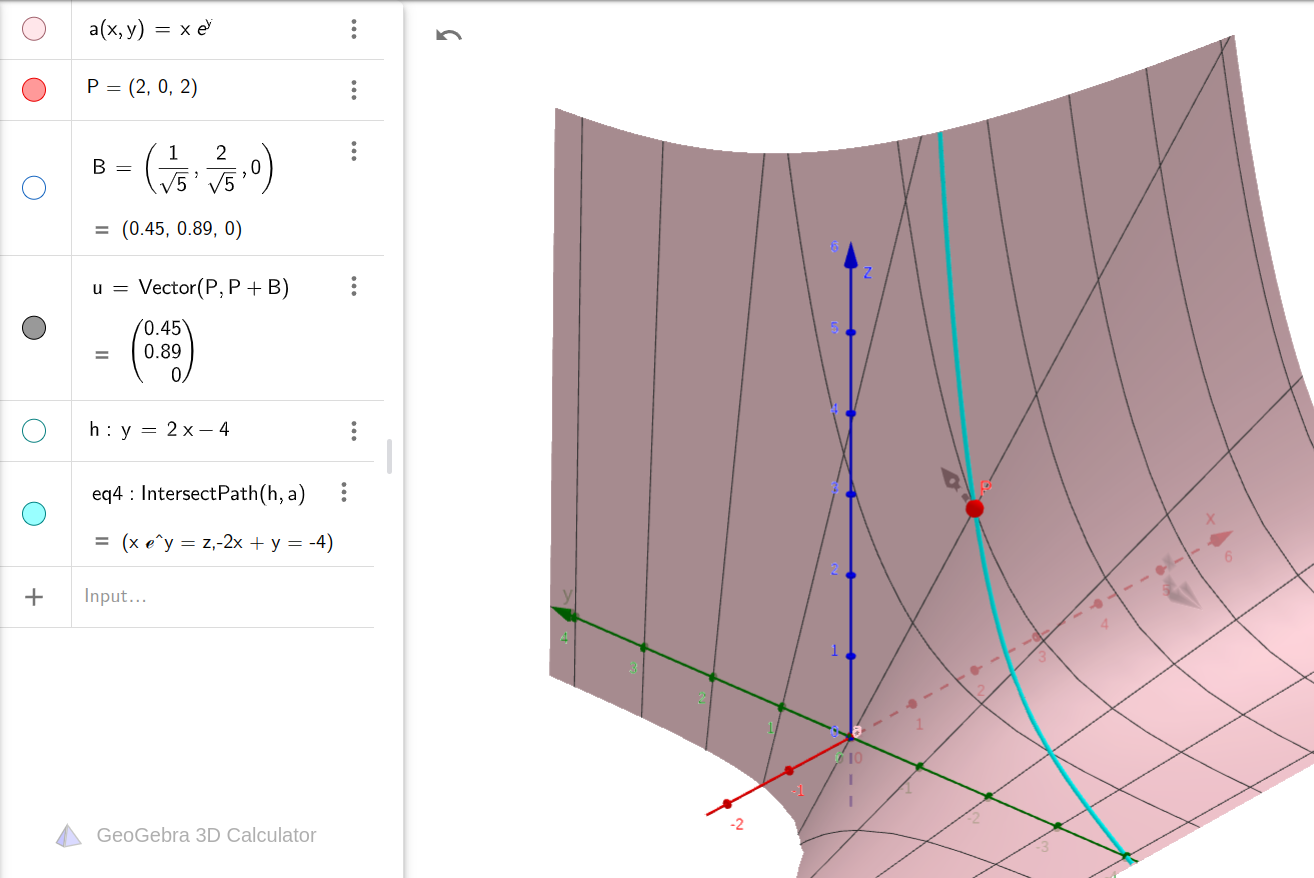
\includegraphics[width=0.95\textwidth]{gradiente-massima-pendenza.png}
\end{center}

\pagebreak
\subsubsection{Derivazione di funzioni composte}

\teorema{Derivazione della funzione composta}{
Supponiamo \(\gamma(t)\) derivabile \(\forall t \in I\), ovvero, \(\gamma'(t) = (\gamma_1'(t),\ldots,\gamma_n'(t)) \quad \forall t \in I\).

Supponiamo inoltre che, data \(f: A \subseteq \Rn \rightarrow \R \), \(f\) sia differenziabile in \(\gamma(t)\).

Allora, la funzione composta \(F: I \rightarrow \R \) che associa \(t \mapsto (f \circ \gamma)(t) = f(\gamma(t)) \), è derivabile in \(t\).

Inoltre vale:
\[
F'(t) = \prods{\nabla f(\gamma(t))}{\gamma'(t)} = \sum^{n}_{i=1} \frac{\partial f}{\partial x_i}(\gamma(t)) \cdot \gamma_i'(t)
\]

}

\begin{proof}
    \( \)

    \textit{Nota: nella seguente dimostrazione, tutte le variabili come \(h\) e \(t\), sono dei vettori.}

    Dimostriamo che \(F\) è derivabile, ovvero che esiste finito il limite del rapporto incrementale:

    \[
        \frac{F(t+h) - F(t)}{\norm{h}}  = \frac{f(\gamma(t+h)) - f(\gamma(t))}{\norm{h}} = \frac{\prods{\nabla f(\gamma(t+h))}{\gamma(t+h) - \gamma(t)} + o(\norm{\gamma(t+h) - \gamma(t)})}{\norm{h}}
    \]

    L'ultimo passaggio deriva dal fatto che, per ipotesi, \(f\) è differenziabile in \(\gamma(t)\), e inoltre stiamo ragionando per \(h \to 0\)

    Vediamo cosa succede per \(h \rightarrow 0\) alle singole parti:
    \begin{enumerate}
        \item
              \[\lim_{ h \to 0 } \frac{\gamma(t+h) - \gamma(t)}{\norm{h}} = \gamma'(t) \hspace{19em}\]

        \item
              \[
                  \lim_{ h \to 0 } \frac{o(\norm{\gamma(t+h) - \gamma(t)})}{\norm{h}} = \lim_{ h \to 0 } {\frac{o(\norm{\gamma(t+h) - \gamma(t)})}{\norm{h}}} \cdot {\frac{\norm{\gamma(t+h) - \gamma(t)}}{\norm{\gamma(t+h) - \gamma(t)}}} =
              \]
              \[
                  = \lim_{ h \to 0 } \underbrace{\frac{o(\norm{\gamma(t+h) - \gamma(t)})}{\norm{\gamma(t+h) - \gamma(t)}}}_\text{\(0\) per definizione di o-piccolo} \cdot \underbrace{\frac{\norm{\gamma(t+h) - \gamma(t)}}{\norm{h}}}_\text{quantità finita} = 0
              \]
              Quantità finita perché:
              \[
                  \lim_{ h \to 0 } \frac{\norm{\gamma(t+h) - \gamma(t)}}{\norm{h}} = \lim_{ h \to 0 } \sqrt{ \sum^{n}_{i=1} {\left(\frac{\gamma_i(t+h) - \gamma_i(t)}{\norm{h}}\right)}^{2} } = \lim_{ h \to 0 } \sqrt{\sum^{n}_{i=1} {( \gamma_i'(t))}^{2}} = \norm{\gamma'(t)} > 0
              \]
    \end{enumerate}
    Dunque:
    \[
        \lim_{ h \to 0 } \frac{F(t+h) - F(t)}{\norm{h}} = \prods{\nabla f(\gamma(t))}{\gamma'(t)} \impliedby \text{tesi}
    \]
\end{proof}

\filbreak{}
\subsubsection*{Esercizio}

Derivare la seguente funzione composta \( f(\gamma(t))\) con:

\[
    f(x,y)= xe^{y}
\]
\[
    \gamma(t) = (x(t), y(t)) = (\cos (t) , \sin (t))
\]

\[
    F(t) = (f \circ \gamma) (t) = f(\gamma(t)) = \cos (t) e ^{\sin (t)}
\]

le derivate parziali sono:

\[
    \nabla f(x,y) = \left( \frac{\partial f}{\partial x}, \frac{\partial f}{\partial y} \right) = (e^{y}, xe^{y})
\]

\[
    \nabla f(\gamma(t)) = (e ^{\sin (t)}, \cos (t) e ^{\sin (t)})
\]

da cui:

\[
    F'(t) = \langle \nabla f(\gamma(t)), \gamma'(t) \rangle
\]

\[
    \gamma'(t) = (-\sin (t), \cos (t))
\]

quindi:

\[
    F'(t) = \left[ e ^{\sin(t)} (- \sin (t)) \right] + \left[ \cos (t) e ^{\sin (t)}\cos (t) \right] = e^{\sin(t)} \left( \cos^{2}(t) -\sin(t) \right)
\]

\pagebreak
\subsubsection{Derivate successive alla prima}

Sia \(f: A \subseteq \Rn  \rightarrow \R \), con \(A\) aperto e \(f\) derivabile su \(A\)

Siano inoltre ben definite le derivate \(\frac{\partial f}{\partial x_i}(x,y) ~\forall i=1,\ldots,n\)

Definiamo cosa significa derivare ulteriormente questa funzione \(f\):

\defn{Derivate seconde}{ Se \(\exists \) sono della forma:

    \[
        \frac{\partial}{\partial x_j} \left( \frac{\partial f}{\partial x_i}(\ux) \right)(\ux)= \frac{\partial^{2} f}{\partial x_i \partial x_j}(\ux) = f_{x_i x_j}(\ux)
    \]

    e si ottengono al variare di \(i,j\) da \(1\) a \(n\).
}

\defn{Matrice Hessiana}{Attraverso le derivate seconde si ottiene una matrice \(n\times n\) che ha come elementi tutte le derivate seconde. Questa è chiamata matrice Hessiana e si indica con:

    \[
        Hf= \begin{bmatrix}
            \frac{\partial^{2} f}{\partial x_1 \partial x_1} & \frac{\partial^{2} f}{\partial x_1 \partial x_2} & \cdots & \frac{\partial^{2} f}{\partial x_1 \partial x_n} \\
            \frac{\partial^{2} f}{\partial x_2 \partial x_1} & \cdots                                           & \cdots & \cdots                                           \\
            \cdots                                           & \cdots                                           & \cdots & \cdots                                           \\
            \frac{\partial^{2} f}{\partial x_n \partial x_1} & \cdots                                           & \cdots & \frac{\partial^{2} f}{\partial x_n \partial x_n}
        \end{bmatrix} = \begin{bmatrix}
            f_{x_1 x_1} & f_{x_1 x_2} & \cdots & f_{x_1 x_n} \\
            f_{x_2 x_1} & \cdots      & \cdots & \cdots      \\
            \cdots      & \cdots      & \cdots & \cdots      \\
            f_{x_n x_1} & \cdots      & \cdots & f_{x_n x_n}
        \end{bmatrix}
    \]

}

\textbf{Nota:} se la matrice Hessiana è ben definita, ovvero esistono tutte le derivate seconde, allora \(f\) si dice \textbf{derivabile 2 volte} in \(\ux_0\).

\defn{Derivate Pure}{
    Sono quelle che derivano per la stessa variabile, ovvero quelle che stanno sulla diagonale della matrice Hessiana:

    \[
        \frac{\partial^{2} f}{\partial x_i \partial x_i} = \frac{\partial^{2} f}{{(\partial x_i)}^{2}}
    \]

}

\defn{Derivate Miste}{
    Sono quelle che derivano per variabili diverse:

    \[
        \frac{\partial^{2} f}{\partial x_i \partial x_j}
    \]
}

\subsubsection*{Esempio matrice Hessiana per n=2}

\[
    Hf(x,y) = \begin{bmatrix}
        \displaystyle\frac{\partial^{2} f}{\partial x^{2}}(x,y)        & \displaystyle\frac{\partial^{2} f}{\partial x \partial y}(x,y) \\[5mm]
        \displaystyle\frac{\partial^{2} f}{\partial y \partial x}(x,y) & \displaystyle\frac{\partial^{2} f}{\partial y^{2}}(x,y)
    \end{bmatrix}
\]

\subsubsection*{Esercizio Matrice Hessiana}

Scrivere la matrice Hessiana di \(f(x,y)= xe ^{y}\):

Partiamo derivando per x:

\[
    f_x(x,y) = e ^{y}
\]

dunque:

\[
    f_{xx}(x,y) = 0
\]
\[
    f_{xy}(x,y) = e^{y}
\]

Partendo poi derivando per y:

\[
    f_y(x,y) = x e^{y}
\]

dunque:

\[
    f_{yx}(x,y) = e^{y}
\]
\[
    f_{yy}(x,y) = x e^{y}
\]

La matrice Hessiana di \(f(x,y)\) è dunque:

\[
    Hf = \begin{bmatrix}
        0      & e ^{y}  \\
        e ^{y} & x e^{y}
    \end{bmatrix}
\]

\pagebreak
\subsubsection{Teorema di Schwarz}

\teorema{Schwarz}{
    Sia \(f: A \subseteq \Rn  \rightarrow \R \), \(A\) aperto

    Sia, inoltre, \(f\) derivabile due volte su \(A\) in \(\ux_0\), con \(\ux_0 \in A\).

    Se le \(f_{x_i x_j}\), e le \(f_{x_j x_i}\) con \(i \neq j\) sono \textbf{continue} in \(\ux_0\), allora:

    \[
        f_{x_i x_j}(\ux_0) = f_{x_j x_i}(\ux_0)
    \]
}

Quindi, se \(f \in C^{2} (A) \xrightarrow[]{\text{Schwarz}} f_{xy}(x,y) = f_{yx}(x,y) \quad \forall (x,y) \in A\). Inoltre, \(H f(x,y)\) è simmetrica \(\forall (x,y) \in A\), ovvero, \({(Hf(x,y))}^{T}=Hf(x,y)\).

Più in generale, se \(f \in C^{k}(A)\) allora l'ordine di derivazione non conta per le derivate parziali fino all'ordine \(k\).

Vediamo più nel dettaglio cosa succede nel caso di funzioni a due variabili.

\filbreak{}
\subsubsection*{Caso n=2}

Sia \(f: A \subseteq \R^{2} \rightarrow \R \), \(P_0=(x_0,y_0) \in A\);

Sia \(f\) derivabile due volte su \(A\) (quindi esiste la matrice Hessiana);

Se le \(f_{xy}\) e \(f_{yx}\) sono continue in \((x_0,y_0)\), allora \(f_{xy}(x_0,y_0) = f_{yx}(x_0,y_0)\).

\begin{proof}
    Sia \(P_0=(x_0,y_0)\) e \(P=(x,y)\) un punto qualsiasi su \(A\), con \(P \neq P_0\)

    \begin{center}
        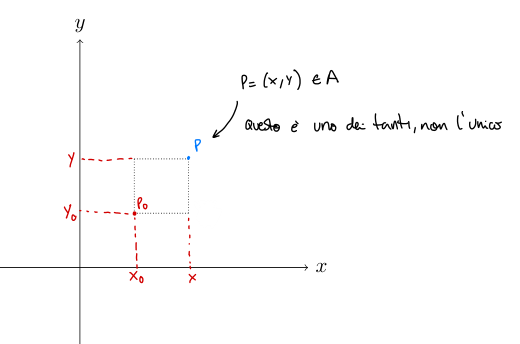
\includegraphics[width=0.55\textwidth]{teorema-di-schwarz-1.png}
    \end{center}

    Consideriamo il valore della funzione nei punti:
    \[
        f(x_0,y_0), f(x,y_0), f(x,y), f(x_0,y)
    \]

    e definiamo le seguenti funzioni che fissano una delle due variabili:
    \[
        F(x) = f(x,y) - f(x,y_0)
    \]
    \[
        G(y)  = f(x,y) - f(x_0,y)
    \]

    Con queste funzioni è evidente la seguente relazione:
    \[
        F(x) - F(x_0) = [f(x,y) - f(x,y_0)] - [f(x_0,y) -f(x_0,y_0)] = f(x,y) - f(x,y_0) - f(x_0,y) + f(x_0,y_0)
    \]
    \[
        G(y) - G(y_0) = [f(x,y) - f(x_0,y)] - [f(x,y_0) -f(x_0,y_0)] = f(x,y) - f(x_0,y) - f(x,y_0) + f(x_0,y_0)
    \]
    Quindi abbiamo che:
    \[
        F(x) - F(x_0) = G(y) -G(y_0)
    \]
    \filbreak{}
    Proviamo quindi a sviluppare le due parti singolarmente:
    \begin{itemize}
        \item Applico il teorema di Lagrange a \(F(x)\) nell'intervallo di estremi \((x_0, x)\), quindi si ha che esiste un punto \(x_1\) in questo intervallo per cui:

              \[
                  F(x)- F(x_0) = F'(x_1) (x-x_0)
              \]
              e dato che, \(F(x_1)=f(x_1,y)-f(x_1,y_0)\), posso arrivare a dire che:
              \[
                  F'(x_1) (x-x_0) = [f_x(x_1,y) - f_x(x_1,y_0) ] (x -x_0)
              \]

              Sappiamo che \(f\) è derivabile due volte, posso quindi applicare nuovamente Lagrange a \(f_x(x_1,y)\) nell'intervallo di estremi \((y_0,y)\). Quindi \(\exists y_1\) nell'intervallo tale che:

              \[
                  f_x(x_1,y) - f_x(x_1,y_0) = \frac{\partial }{\partial y}(f_x(x_1,y_1))(y-y_0) = f_{xy}(x_1,y_1)(y-y_0)
              \]

              quindi abbiamo fatto vedere che:

              \[
                  F(x)- F(x_0) = [f_{xy}(x_1,y_1)] (x-x_0) (y-y_0)
              \]
        \item Analogamente per \(G(y)\) applico Lagrange, quindi \(\exists y_2\) nell'intervallo \((y,y_0)\) tale che:

              \[
                  G(y) -G(y_0) = G'(y_2) (y-y_0) = [f_y(x,y_2) - f_y(x_0,y_2)] (y-y_0)
              \]

              applico nuovamente Lagrange a \(f_y(x,y_2)\) nell'intervallo \((x,x_0)\). Quindi \(\exists x_2 \in (x,x_0)\) t.c.:
              \[
                  f_y(x,y_2) - f_y(x_0,y_2) = f_{yx}(x_2,y_2)(x-x_0)
              \]
              infine quindi:
              \[
                  G(y) -G(y_0) = f_{yx}(x_2,y_2)(x-x_0)(y-y_0)
              \]
    \end{itemize}
    Ora, essendo \(F(x) - F(x_0) = G(y) - G(y_0)\), segue che:
    \[
        f_{xy}(x_1,y_1)(x-x_0)(y-y_0) = f_{yx}(x_2,y_2)(x-x_0)(y-y_0)
    \]

    e dato che per l'ipotesi iniziale \(P \neq P_0\), segue che \((x,y) \neq (x_0,y_0)\). Possiamo quindi semplificare le quantità non nulle, ovvero:
    \[
        f_{xy}(x_1,y_1) = f_{yx}(x_2,y_2)
    \]

    dove \((x_1,y_1)\) e \((x_2,y_2)\) stanno nell'intervallo del rettangolo tratteggiato del grafico iniziale.

    \filbreak{}
    Passando al limite per \(P \rightarrow P_0\), succede che:
    \[
        (x,y) \rightarrow (x_0,y_0)
    \]
    \[
        (x_1,y_1) \rightarrow (x_0,y_0)
    \]
    \[
        (x_2,y_2) \rightarrow (x_0,y_0)
    \]

    inoltre, ricordo che per il teorema di Lagrange:
    \[y_0 < y_1, y_2 < y\]
    \[x_0 < x_1, x_2 < x\]

    essendo, per ipotesi iniziale, le funzioni \(f_{xy},f_{yx}\) continue in \(P_0=(x_0,y_0)\), passando al limite di \(P \rightarrow P_0\) si ha dunque:
    \[
        f_{xy}(x_0,y_0) = f_{yx}(x_0,y_0)
    \]
\end{proof}

\pagebreak
\begin{proof} \textbf{Alternativa con integrali doppi}

    Sia un generico rettangolo \(R = [a,b]\times [c,d]\)

    Integro \(f_{xy}(x,y)\):

    \begin{spreadlines}{2mm}
        \begin{align*}
            \int_c^d \int_a^b {f_{yx}(x,y)} \diff{x}\diff{y} & = \int_c^d \int_a^b {(f_y(x,y))}_x \diff{x}\diff{y}               \\
                                                             & = \int_c^d \left[ f_y(b,y) - f_y(a,y) \right] \diff{y}            \\
                                                             & = \left[ f(b,d) - f(b,c) \right] + \left[ f(a,d) - f(a,c) \right]
        \end{align*}
    \end{spreadlines}

    Adesso vediamo l'altro integrale di \(f_{yx}(x,y)\) (si inverte l'integrale con il teorema di Fubini che presuppone che la funzione sia continua):

    \[
        \int_c^d \int_a^b f_{xy} \diff{x}\diff{y} \overset{\text{Teorema di Fubini}}{=} \int_a^b \int_c^d {(f_x)}_y \diff{y}\diff{x} =
    \]

    \[
        =\int_a^b \left[ f_x(x,d) - f_x(x,c) \right] \diff{x}  = [f(b,d) - f(a,d)] + [f(b,c) - f(a,c)]
    \]

    e quindi \(f_{xy}(x,y) = f_{yx}(x,y)\):

    \[
        f(b,d) - f(b,c) - f(a,d) + f(a,c) = f(b,d) - f(a,d) - f(b,c) + f(a,c)
    \]

    Questo funziona per ogni rettangolo che pongo infatti:

    \[
        \int_c^d \int_a^b f_{yx} \diff{x}\diff{y} =  \int_c^d \int_a^b f_{xy} \diff{x}\diff{y}
    \]

    Quindi la loro differenza deve essere 0:

    \[
        \iint_R \underbrace{{(f_{yx} - f_{xy})}}_\text{continue} \diff{x}\diff{y} = 0
    \]

    Vale perché essendo le funzioni continue, se supponiamo per assurdo che la differenza sia positiva in un certo punto \(\ux_0\) allora la funzione è positiva anche in un piccolo rettangolo intorno a quel punto (per la continuità) ma questo è assurdo perché nel rettangolo la differenza delle due funzioni è 0.

    Quindi, il teorema di Schwarz funziona proprio per il fatto che le funzioni sono continue.

\end{proof}

\pagebreak
\subsubsection*{Esempio su Schwarz}

Usando il teorema di Schwarz, dire se la seguente funzione, \(f: \R^{2} \rightarrow \R \), è derivabile più di una volta, e in che punti:

\[
    f(x,y)=\begin{cases}
        0                                               & \text{se \((x,y) = (0,0)\)}    \\
        \displaystyle \frac{yx^{3}-xy^{3}}{x^{2}+y^{2}} & \text{se \((x,y) \neq (0,0)\)}
    \end{cases}
\]

Vediamo lo svolgimento per punti:
\begin{itemize}
    \item Prima cosa, verifichiamo che \(f(x,y)\) sia continua in \((0,0)\), ovvero che:

          \[
              \lim_{ (x,y) \to (0,0) } f(x,y)=f(0,0) = 0
          \]

          Passiamo in coordinate polari:
          \begin{align*}
              \frac{\rho\sin(\theta)\rho^3\cos^3(\theta) - \rho\cos(\theta)\rho^3\sin^3(\theta)}{\rho^2\cos^2\theta + \rho^2\sin^2\theta} & = \frac{\rho^4\left[ \sin(\theta)\cos^3(\theta) - \cos(\theta)\sin^3(\theta) \right]}{\rho^2}                \\
                                                                                                                                          & = \rho^2\sin(\theta)\cos(\theta) \left[ \cos^2(\theta) - \sin^2(\theta) \right] \xrightarrow[\rho \to 0]{} 0 \\
          \end{align*}
          Verifichiamo con il teorema del confronto:
          \begin{align*}
              \Big| \rho^2\sin(\theta)\cos(\theta) \left[ \cos^2(\theta) - \sin^2(\theta) \right] \Big| & \le \Big| \rho^2\sin(\theta)\cos(\theta) \left[ \cos^2(\theta) + \sin^2(\theta) \right] \Big| \\
                                                                                                        & \le \rho^2 \Big| \sin(\theta)\cos(\theta) \Big|                                               \\
                                                                                                        & \le \rho^2
          \end{align*}
          e dato che \(\rho^2 \xrightarrow[\rho \to 0]{} 0\), abbiamo verificato che \(f(x,y) \xrightarrow[(x,y) \to (0,0)]{} 0\), ovvero che \(f\) è continua in \((0,0)\).

    \item Ora, verifichiamo che anche le derivate parziali \(f_x(x,y)\) e \(f_y(x,y)\) siano continue in \((0,0)\):
          \begin{align*}
               & f_x(0,0) = \lim_{ h \to 0 } \frac{f(0+h,0) - f(0,0)}{h} = \lim_{ h \to 0 } \left( \frac{h^{3}\cdot0 - h\cdot 0}{h^{2}+0} - 0 \right) \cdot  \frac{1}{h} = \lim_{ h \to 0 } \frac{0}{h} = 0 \\[2mm]
               & f_y(0,0) = \lim_{ h \to 0 } \frac{f(0,0+h) - f(0,0)}{h} = \cdots = 0
          \end{align*}

          \filbreak{}
    \item Calcoliamo le derivate parziali per \((x,y) \neq (0,0)\):
          \begin{align*}
               & f_x(x,y) = \frac{(3x^{2}y-y^{3})(x^{2}+y^{2})-(x^{3}y-xy^{3})(2x)}{{(x^{2}+y^{2})}^{2}} = \frac{x^{4}y+4x^{2}y^{3}-y^{5}}{{(x^{2}+y^{2})}^{2}} \\[2mm]
               & f_y(x,y) = \cdots = \frac{-xy^{4}-4x^{3}y^{2}+x^{5}}{{(x^{2}+y^{2})}^{2}}
          \end{align*}

    \item ricordando da sopra che \(f_x(0,0)=0=f_y(0,0)\), calcoliamo le derivate seconde in \((0,0)\):
          \[
              f_{xy} (0,0) = \lim_{ k \to 0 } \frac{f_x(0,0+k) - f_x(0,0)}{k} = \lim_{ k \to 0 } \frac{ \left( \frac{-k^{5}}{k^{4}} \right) - (0)}{k} = \lim_{ k \to 0 } - \frac{k}{k} = -1
          \]
          \[
              f_{yx}(0,0) = \lim_{ k \to 0 } \frac{f_y(0+k,0) - f_y(0,0)}{k} = \lim_{ k \to 0 } \frac{ \left( \frac{k^{5}}{k^{4}} \right) - (0)}{k} = \lim_{ k \to 0 } \frac{k}{k} = 1
          \]
\end{itemize}

Possiamo quindi dire che la funzione \(f(x,y)\) è derivabile due volte su \((0,0)\), ma che \(f(x,y) \notin C^2(A)\). Questo perché le derivate seconde sono diverse e quindi per il teorema di Schwarz le derivate seconde non sono continue in \((0,0)\).
